\documentclass{scrartcl}
\usepackage{graphicx}
\usepackage{float}
\usepackage[spanish]{babel}
\usepackage{hyperref} 
\graphicspath{ {img/} }
\setlength{\parskip}{\baselineskip}

\title{Diseño Arquitectónico de una Aplicación}
\subtitle{\large PAMN - Programación de Aplicaciónes Moviles Nativas}
\author{Chamil José Cruz Razeq}

\begin{document}
    \maketitle
    \thispagestyle{empty}
    \newpage
    \tableofcontents
    \newpage

    \section{Introducción}
        Este documento recoge los resultados de la tárea propuesta para la
         confección de un diseño arquitectónico de una aplicación. Para ello
         se establecerá un dominio y arquitectura, presentando sus características
         principales acompañadas de un diagrama.

        Todas las tareas propuestas se encuentran disponibles en el siguiente
         repositorio de \href{https://github.com/chamilstudy/ulpgc_pamn_labs}{GitHub}.
    
    \section{Dominio}
        Aplicación alternativa al servicio web del cabildo para la solicitud de
         permisos e información sobre las areas recreativas.
        
        Como funcionalidades comunes con el servicio web encontramos:
        \begin{itemize}
            \item Listado de areas disponibles.
            \item Información sobre las instalaciones y estado de cada área.
            \item Solicitud de permisos para su uso (hornos de piedra, acampadas, caravanas...).
        \end{itemize}

        Como funcionalidades adicionales ofrecidas por la aplicación:
        \begin{itemize}
            \item Búsqueda de areas facilitada a través de filtros.
            \item Historial de solicitudes.
            \item Información en tiempo real del estado de las áreas y sus instalaciones.
            \item Advertencias en tiempo real en situaciones de emergencia.
        \end{itemize}
    
    \section{Arquitectura}
        Para el desarrollo del dominio anterior se ha seleccionado la arquitectura MVVM
         \footnote[1]{El patrón MVVM ayuda a separar limpiamente la lógica de presentación y negocios de
         una aplicación de su interfaz de usuario \cite[MVVM]{msmvvm}.} por su afinidad con el desarrollo
         para aplicaciones moviles y atractivas características que facilitan el desarrollo y la realización
         de pruebas [Figura 1].

         \begin{figure}
            \centerline{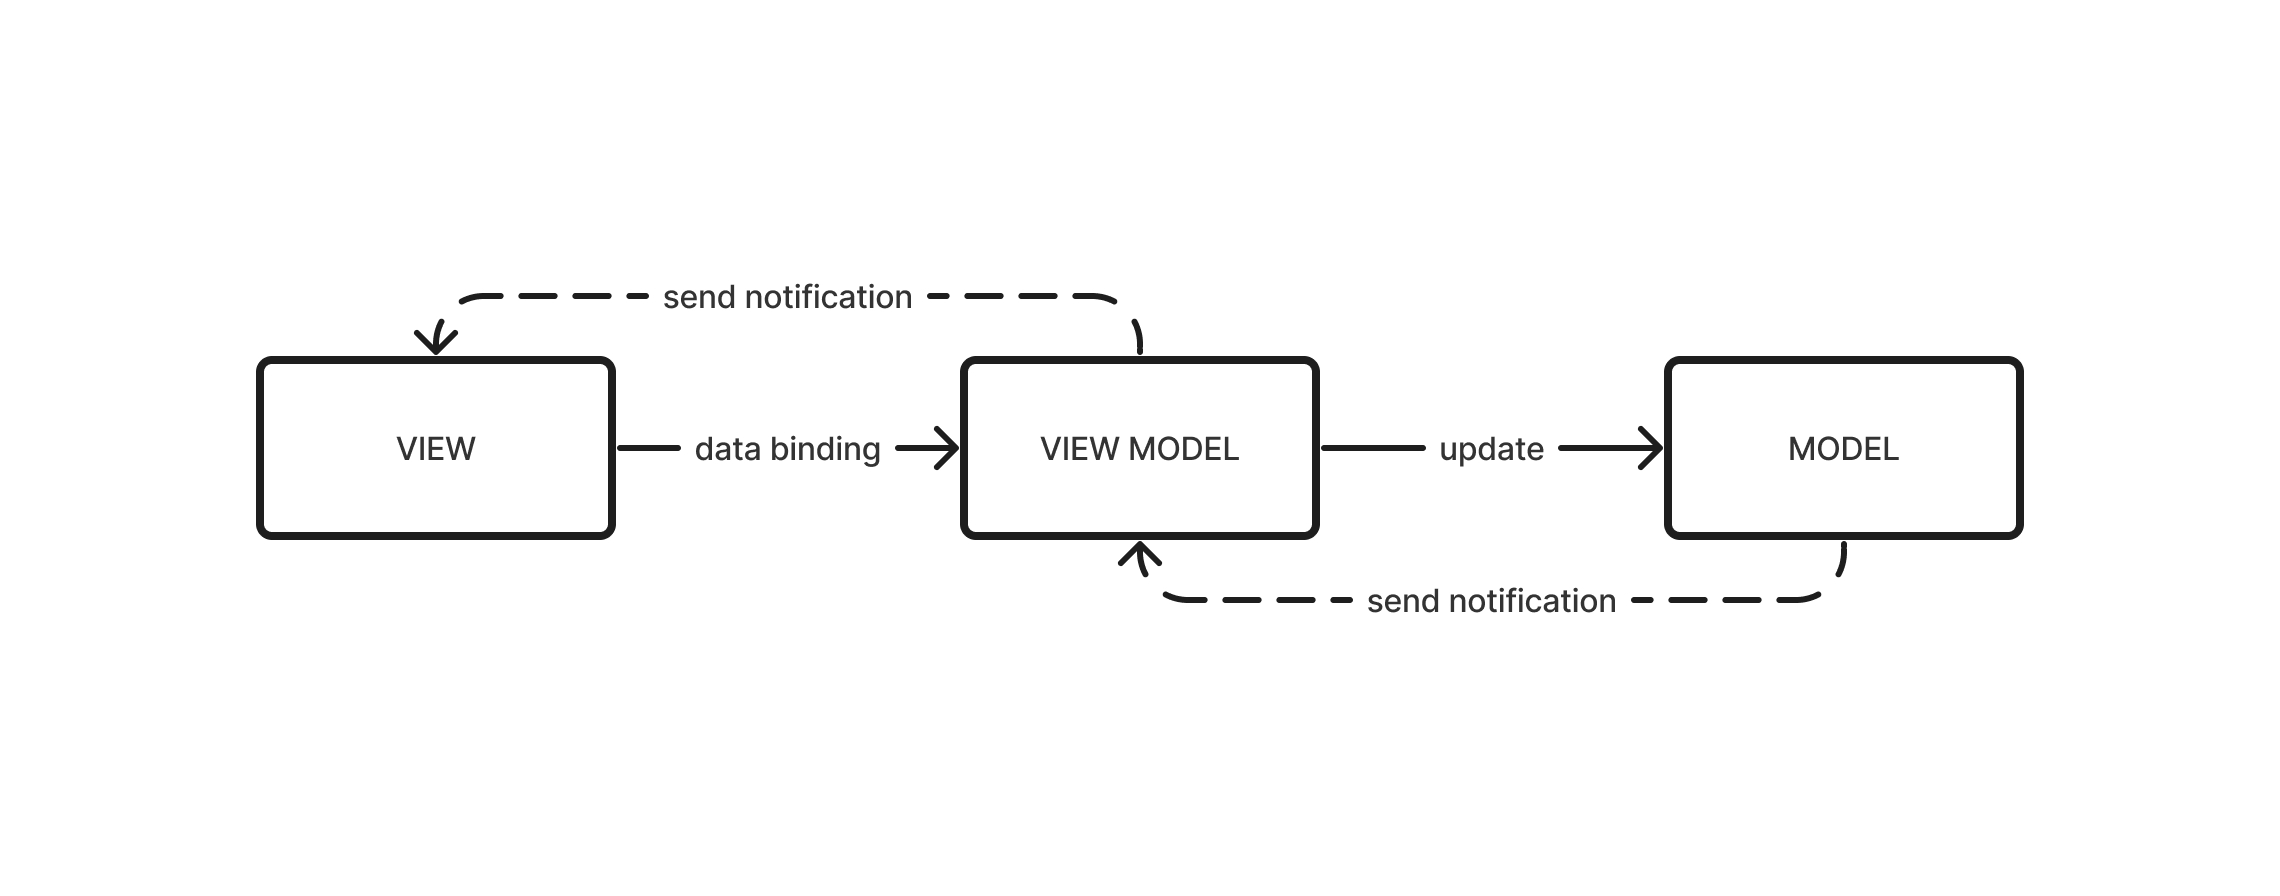
\includegraphics[scale=0.4]{mvvmdiagram}}
            \caption{Diagrama de MVVM}
            \label{fig:mvvmdiagram}
         \end{figure}

        Para el dominio planteado, podemos identificar:

        \begin{itemize}
            \item VistaAreas, ModeloVistaAreas y ModeloAreas: con información reducida
                   de cada area [Figura 2].
            \item VistaAreaEspecifica, ModeloVistaAreaExpecifica y ModeloAreaEspecifica:
                   con información detallada de un área especificada.
            \item VistaSOS, ModeloVistaSOS y ModeloSOS: con información de los medios de
                   seguridad y emergencias.
            \item VistaSolicitud, ModeloVistaSolicitud y ModeloSolicitud: gestionando el
                   formulario de solicitudes de uso de áreas recreativas.
            \item VistaSolicitudes, MOdeloVistaSolicitudes y ModeloSolicitudes: gestionando
                   las solicitudes de uso de áreas recreativas.
        \end{itemize}

        \begin{figure}
            \centerline{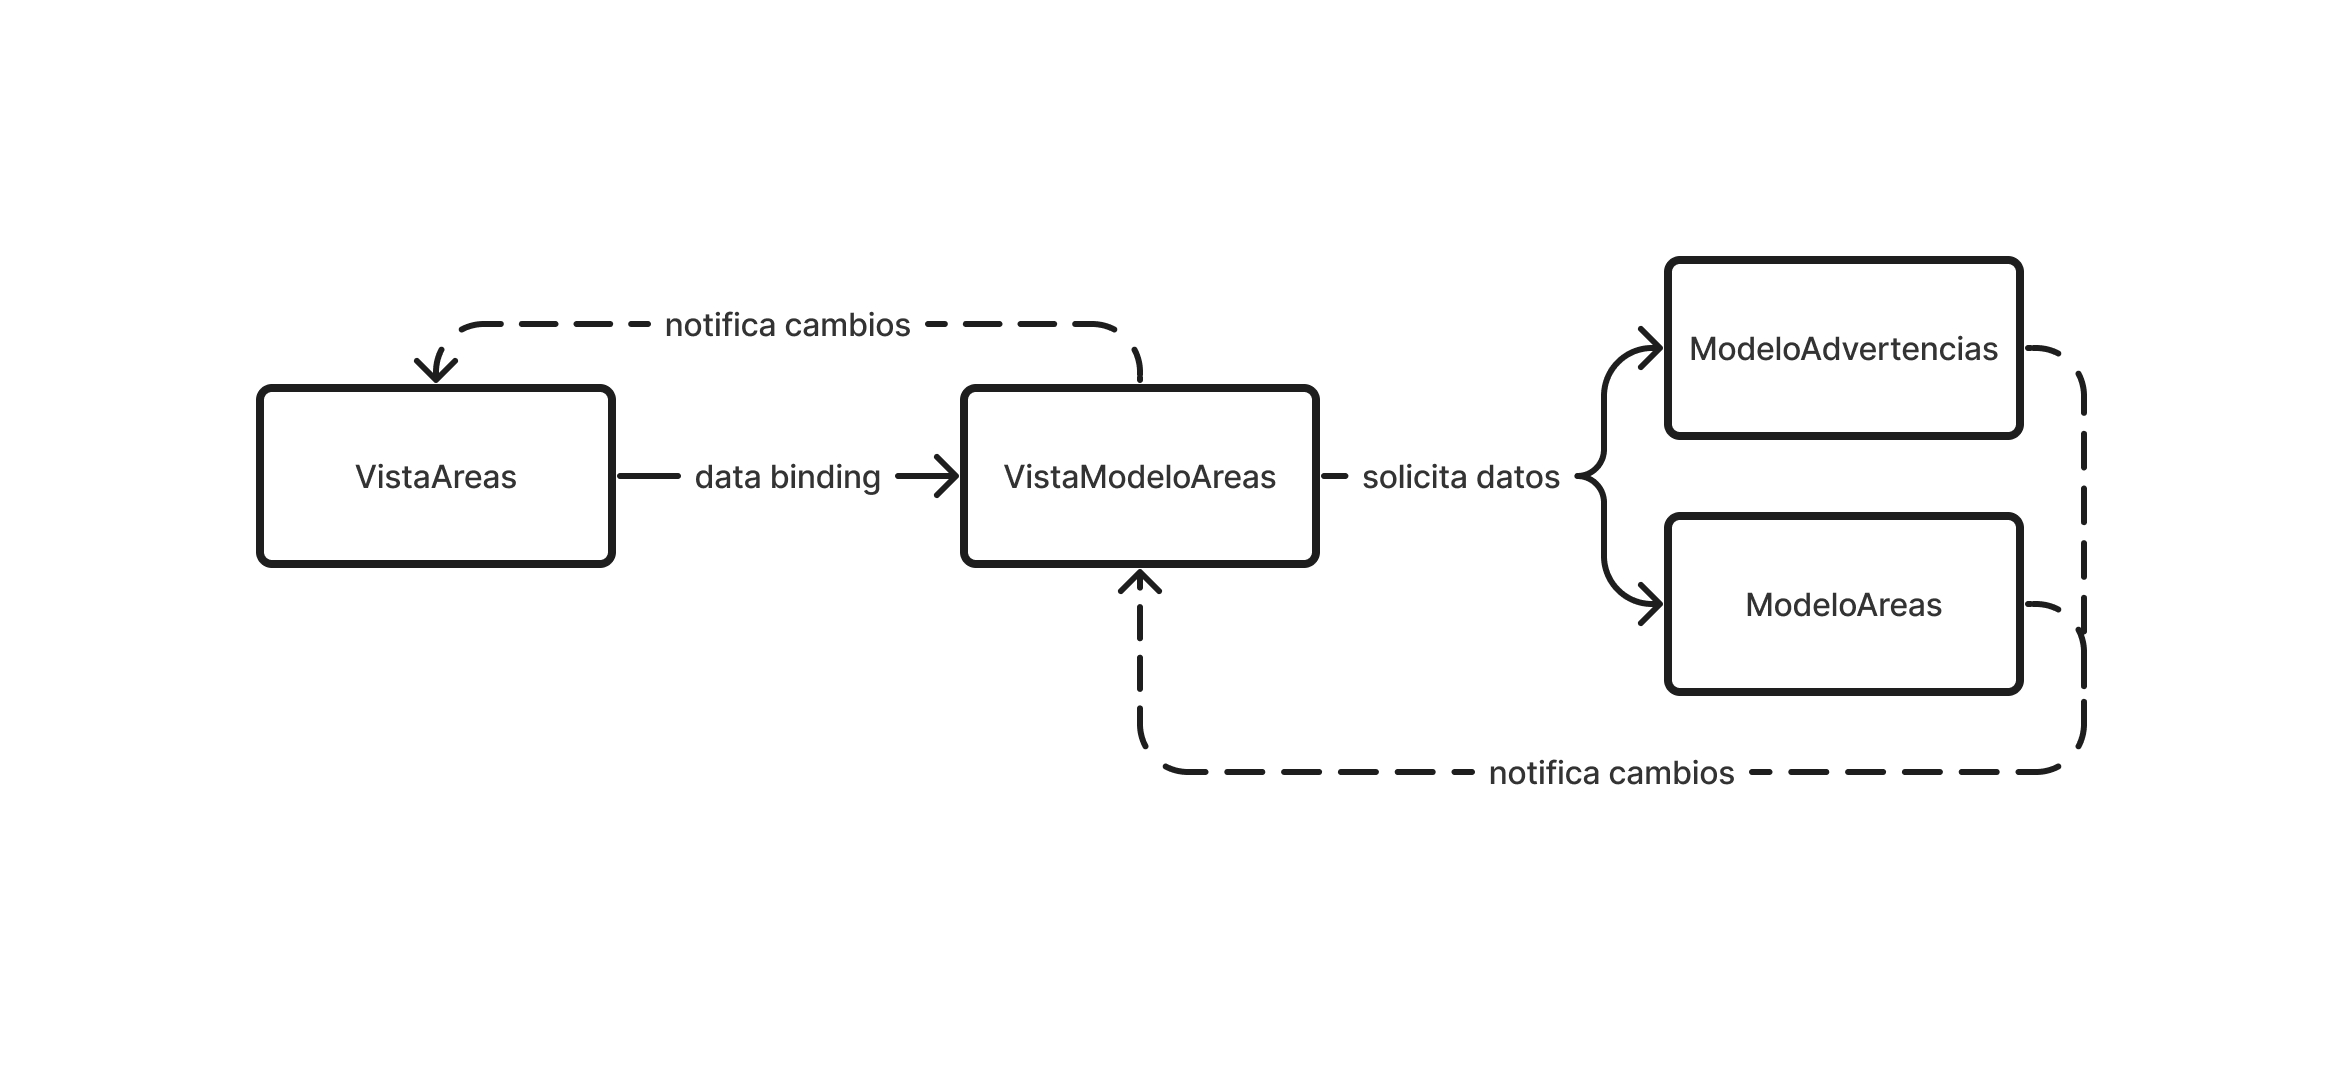
\includegraphics[scale=0.4]{areasdiagram}}
            \caption{Diagrama de funcionalidad de áreas}
            \label{fig:areasdiagram}
         \end{figure}
    
    \newpage
    \section{Casos de Uso}
        Tomando como referencia la [Figura 2] podemos identificar dos casos de uso
        fundamentales para la aplicación propuesta.

        \begin{itemize}
            \item El usuario puede ver las areas recreativas disponibles: en este caso
                    siguiendo lo observado en [Figura 2], el usuario (usando o no filtros),
                    tendrá a su disposición una lista de areas con información esencial. 
                    Siguiendo la arquitectura MVVM, el "Modelo" proveera con la información
                    actualizada al "ModeloVista" que notificara a la "Vista". En caso de que
                    el usuario interactue con el sistema, se procedera a solicitar la información
                    actualizada al "Modelo".
            \item El usuario puede seleccionar y ver información adicional de un area: en este
                   caso la "Vista" el "ModeloVista" y el "Modelo" cambián al caso de "AreaEspecifica".
                   En este contexto solo se hará uso de la información provista por el "Modelo" y los
                   cambios que se hayan podido producir sin interaccción del usuario.
        \end{itemize}

    
    \section{Conclusion}
        El modelo MVVM demuestra ser una arquitectura versatil, idonea para cualquier proyecto de
         desarrollo movil. En nuestro caso facilitaría no solo la creación de los diferentes
         componentes del software, sino que tambien facilitaría la confección de pruebas (a traves del
         "ModeloVista"). Las principales ventajas de MVVM frente a otros modelos son la posibilidad de
         realización de pruebas facilmente (frente a MVC) y su sencillez, dado el dominio planteado, 
         ya que otros modelos plantean un manejo mas estricto de la información (frente a MVI).
    \newpage
    \begin{thebibliography}{}
        \bibitem{msmvvm} Microsoft Learn - https://learn.microsoft.com/es-es/dotnet/architecture/maui/mvvm
    \end{thebibliography}

\end{document}
